\documentclass[11pt]{article}
\usepackage[a4paper,margin=1in]{geometry}
\usepackage{subfiles}
\usepackage{amsmath,amssymb,bm}
\usepackage{hyperref}
\usepackage{booktabs}
\usepackage{array}
\usepackage{mathtools}
\usepackage{graphicx}

\title{Appendix 18 (to main theory): Pressure-History Process Time, Operational Time, and Rate Conversion}
\author{}
\date{}

\begin{document}
\let\phi\varphi
\maketitle

\section*{Purpose and scope}
This appendix records in one place a time concept that is already used
implicitly across the ISPG framework but had not previously been isolated
as a standalone result.  The clock-rate postulate of the bi-conformal
geometry implies that pressure-controlled matter-sector processes do not accumulate history
according to the naive present-day clock alone.  Instead, they accumulate
according to a pressure-weighted process time.

The purpose of the appendix is sixfold:
\begin{enumerate}
\item define the pressure-history process time from the basic clock law;
\item distinguish it sharply from the FLRW cosmic time used in Appendix~9;
\item formalize the status of the quiescent medium as an operationally
  timeless sector;
\item derive the redshift integral and quantitative bounds for cumulative
  process histories;
\item state a precise rate-conversion and no-double-counting rule; and
\item extract the asymptotic consequence for weakening cosmological activity.
\end{enumerate}

No new field, no second metric, and no modification of the linear-cosmology
sector are introduced here.  The result is an operational consequence of
the already-established pressure ontology.

\section{Operationally timeless medium and onset of measurable time}
\label{sec:op_time_app18}

The ISPG framework does not require time to be assigned as an abstract label
independently of physical oscillators.  In the companion quantum
interpretation, a region with no localized resonance contains no atom,
particle, or clock and therefore no operational procedure for defining
proper time.  Such a region is not assigned a second hidden time variable;
it is \emph{operationally timeless}.

This claim has a precise mathematical anchor in the companion quantum
interpretation.  The quiescent medium is characterized by two
gauge-invariant conditions:
\begin{equation}
  \nabla\phi = 0
  \qquad\text{and}\qquad
  \text{no localized resonant excitation.}
  \label{eq:quiescent_def}
\end{equation}
Without a resonant oscillator---an atom, a particle, a clock---there is no
operational procedure for measuring proper time, regardless of the
background value of $\phi$.  ``Operationally timeless'' is the shorthand
for this condition; it is not a statement about $\phi$ taking a particular
value, but about the absence of the physical structures that give time its
operational meaning.

Equivalently, the medium is not assigned its own hidden clock that can run
fast or slow.  The factor $d\tau=e^{\phi/2}dt$ is defined only for
localized resonant processes and for instruments built from them.

This gives a sharp reading of the quiescent medium:
\begin{itemize}
\item before a finite resonant excitation forms, finite clocks and finite
  rulers are not yet operationally defined;
\item when resonant excitations and their tails appear, the medium acquires
  finite pressure deficits, finite oscillation periods, and therefore
  measurable time scales;
\item the observable universe is the finite resonant-excitation sector of an
  otherwise quiescent medium.
\end{itemize}

The role of the present appendix is not to replace FLRW cosmic time by this
operational statement.  Its role is to identify the correct time variable
for \emph{cumulative pressure-controlled matter histories}.

\section{Unified pressure scaling of clocks, rods, mass, and tail emission}
\label{sec:clocklaw_app18}

The ISPG pressure potential is defined by
\begin{equation}
  \phi \equiv \ln\!\left(\frac{P_{\mathrm{stat}}}{P_{\max}}\right),
\end{equation}
so that $\phi=0$ at the asymptotic vacuum normalization
$P_{\mathrm{stat}}=P_{\max}$.

The operational clock-rate postulate gives
\begin{equation}
  d\tau = e^{\phi/2}\,dt,
  \label{eq:clock_app18}
\end{equation}
where $t$ is the coordinate time appearing in the bi-conformal line
element and $\tau$ is the local proper time of physical processes.
Equation~\eqref{eq:clock_app18} is not an auxiliary assumption: it is part
of the construction of the geometry itself (Appendix~3).

The same pressure state also rescales rods reciprocally:
\begin{equation}
  d\ell = e^{-\phi/2}\,d\sigma,
  \label{eq:rod_app18}
\end{equation}
and it rescales the effective particle mass as
\begin{equation}
  m_{\mathrm{eff}} = m_0 e^{\phi/2}.
  \label{eq:meff_app18}
\end{equation}
Since the single-particle resonant-tail power obeys
\begin{equation}
  \mathcal{P}_{\mathrm{tail}} \propto m_{\mathrm{eff}}^4,
  \label{eq:Ptail_scaling_app18}
\end{equation}
one immediately obtains
\begin{equation}
  \mathcal{P}_{\mathrm{tail}} \propto e^{2\phi}.
  \label{eq:Ptail_phi_app18}
\end{equation}

\paragraph{Local-to-cosmological extension.}
Equations \eqref{eq:clock_app18}--\eqref{eq:meff_app18} are derived in
Appendix~3 for the static exterior of an isolated source, where $\phi(r)$
is a spatial profile.  The scalings $d\tau\propto e^{\phi/2}$,
$d\ell\propto e^{-\phi/2}$, $m_{\mathrm{eff}}\propto e^{\phi/2}$ follow
from the bi-conformal metric ansatz
$ds^2=-e^{\phi}c^2dt^2+e^{-\phi}d\sigma^2$ and the matter coupling
$S_m[g_{\mu\nu},\psi]$, not from the particular form $\phi=-r_s/r$.

\paragraph{Scope of the substitution.}
In the cosmic-time gauge (Appendix~9, Eq.~\ref{eq:phi0_app18}) the
homogeneous \emph{metric} scalar obeys $\phi_0=0$ by construction, so a
literal application of Eq.~\eqref{eq:clock_app18} with the metric
$\phi$ yields $d\tau=dt$ at the homogeneous level.  What
Eqs.~\eqref{eq:C_clock_app18}--\eqref{eq:C_tail_app18} use is instead
the coarse-grained pressure diagnostic $\phi_{\mathrm{bg}}(z)$ of
Eq.~\eqref{eq:phibg_def_app18}; the same functional form
$e^{\phi/2}$ is \emph{reapplied} to this thermodynamic variable by
postulating that the clock--rod--mass response of the matter sector
tracks the medium pressure state regardless of whether that state is
encoded as a metric profile (isolated source) or as a volume-averaged
thermodynamic variable (cosmological history).  This reuse is not a
consequence of the Appendix~3 derivation: the Appendix~3 argument
establishes the response only for the metric-$\phi$ channel.  The
$\phi_{\mathrm{bg}}$-channel response is a constitutive postulate of
the pressure ontology, logically distinct from the geometric
derivation, and its detailed compatibility with the Einstein--Boltzmann
system (beyond the leading-order decoupling used in
Sec.~\ref{sec:flrw_vs_process_app18}) is the topic of a separate work.

It is useful to collect the scalings into one background-history factor:
\begin{equation}
  \mathcal{C}(z)
  := e^{[\phi_{\mathrm{bg}}(z)-\phi_{\mathrm{bg}}(0)]/2}
  = \left[\frac{P_{\mathrm{stat}}(z)}{P_{\mathrm{stat}}(0)}\right]^{1/2}.
  \label{eq:Cfactor_app18}
\end{equation}
Then the relative background rescalings are
\begin{align}
  \frac{d\tau_{\mathrm{proc}}}{dt} &= \mathcal{C}(z),
  \label{eq:C_clock_app18}\\
  \frac{d\ell(z)}{d\ell(0)} &= \mathcal{C}(z)^{-1},
  \label{eq:C_rod_app18}\\
  \frac{m_{\mathrm{eff}}(z)}{m_{\mathrm{eff}}(0)} &= \mathcal{C}(z),
  \label{eq:C_mass_app18}\\
  \frac{\mathcal{P}_{\mathrm{tail}}^{(\mathrm{pert})}(z)}
       {\mathcal{P}_{\mathrm{tail}}^{(\mathrm{pert})}(0)}
  &= \mathcal{C}(z)^4.
  \label{eq:C_tail_app18}
\end{align}
Equation~\eqref{eq:Cfactor_app18} is therefore the single pressure-history
multiplier that ties together clock rate, rod scale, effective mass, and
tail-emission strength at the perturbative conformal-exponent level.  The
full non-perturbative tail power should be written schematically as
\begin{equation}
  \mathcal{P}_{\mathrm{tail}}^{(\mathrm{np})}
  = \mathcal{F}_{\mathrm{nonpert}}(\phi_{\mathrm{bg}},\ldots)\,
    \mathcal{P}_{\mathrm{tail}}^{(\mathrm{pert})}.
\end{equation}
If $\mathcal{F}_{\mathrm{nonpert}}$ has background-pressure dependence,
the pure $\mathcal{C}(z)^4$ law is modified.  The companion MOND analysis
uses the same background history through the perturbative coupling
enhancement
$\mathcal{E}(z)=\mathcal{C}(z)^4=e^{2[\phi_{\mathrm{bg}}(z)-\phi_{\mathrm{bg}}(0)]}$.

\section{FLRW cosmic time versus process time: resolving the $\phi_0=0$
  tension}
\label{sec:flrw_vs_process_app18}

Appendix~9 fixes the homogeneous FLRW background in the cosmic-time gauge
by requiring $g_{tt}=-1$ along matter-comoving worldlines.  In that gauge
the homogeneous metric mode obeys
\begin{equation}
  \phi_0 = 0,
  \label{eq:phi0_app18}
\end{equation}
so the background Einstein--Boltzmann system is GR-identical.

That statement does \emph{not} erase the pressure-history weighting of
matter-sector processes, because $\phi_0$ and $\phi_{\mathrm{bg}}$
are logically distinct objects:
\begin{enumerate}
\item \textbf{$\phi_0$: the homogeneous metric scalar.}  This is the
  background value of the field that enters $g_{tt}=-e^{\phi}$.  In
  cosmic-time gauge it is forced to vanish at every epoch
  (Eq.~\ref{eq:phi0_app18}).  It is a metric degree of freedom.
\item \textbf{$\phi_{\mathrm{bg}}(z)$: the coarse-grained medium
  pressure diagnostic.}  This is a volume-averaged thermodynamic
  observable of the medium substance:
  \begin{equation}
    \phi_{\mathrm{bg}}(z)
    := \ln\!\left[\frac{\langle P_{\mathrm{stat}}\rangle_V(z)}
                       {P_{\max}}\right],
    \label{eq:phibg_def_app18}
  \end{equation}
  where $\langle P_{\mathrm{stat}}\rangle_V(z)$ denotes the
  volume-averaged static pressure of the medium at redshift $z$.
  This quantity tracks the global thermodynamic state---it decreases
  as irreversible tail emission depletes pressure over cosmic
  history.  It is \emph{not} a second homogeneous metric mode: it
  does not appear in $g_{\mu\nu}$, and in the cosmic-time gauge the
  metric background remains GR-identical to linear order.  Its
  backreaction on the Einstein--Boltzmann system through the
  effective mass
  $m_{\mathrm{eff}} = m_0\,e^{\phi_{\mathrm{bg}}/2}$ is a subleading
  effect on the matter sector in the late-time matter-dominated
  regime considered here and is absorbed into the observational
  definition of the baryon number density; a quantitative assessment
  of the early-universe regime, where this backreaction could become
  relevant, is the topic of a separate work.
\end{enumerate}

\paragraph{Operational analogy.}
The distinction is analogous to the one between a background temperature
$T_{\mathrm{CMB}}(z)$ and the metric.  The CMB temperature is not itself a
metric degree of freedom, although it contributes to $g_{\mu\nu}$
indirectly through the radiation energy density
$\rho_{\mathrm{rad}}\propto T_{\mathrm{CMB}}^{4}$ entering the Friedmann
equations.  In the same way $\phi_{\mathrm{bg}}(z)$ is not a metric mode:
it is a coarse-grained thermodynamic diagnostic of the medium.  Its
indirect contribution to $g_{\mu\nu}$ through the matter sector (via
$m_{\mathrm{eff}}$) is subleading in the late-time matter-dominated regime
considered here; its role as a driver of pressure-controlled process rates is
logically independent of this small gravitational backreaction.

\paragraph{Where $\phi_{\mathrm{bg}}(z)$ comes from.}
The companion quantum paper derives a feedback ODE
$\dot\varepsilon=\lambda n m_0^4 e^{2\phi}$ whose self-consistent
solution yields, at each redshift, the ratio $e^{2\phi(z)}/e^{2\phi(0)}$
as a function of $H(z)$, $\varepsilon(z)/\varepsilon(0)$, and
$(1+z)^\alpha$ (see the companion MOND paper, Eq.~(5.23)).
The present appendix takes this ratio as an \emph{input} and reads off
the process-time weight from it.  Appendix~18 does not independently
determine $\phi_{\mathrm{bg}}(z)$; it only converts a given
pressure-history ratio into the corresponding time weighting.  Any
downstream use of $\tau_{\mathrm{proc}}$ therefore inherits the
closure used to derive $\phi_{\mathrm{bg}}(z)$, and no circularity
arises provided the closure is not itself derived from
$\tau_{\mathrm{proc}}$.  The relevant equation is
\begin{equation}
  \phi_{\mathrm{bg}}(z)-\phi_{\mathrm{bg}}(0)
  = \ln\!\left[\frac{P_{\mathrm{stat}}(z)}{P_{\mathrm{stat}}(0)}\right].
  \label{eq:phibg_app18}
\end{equation}

\paragraph{Inheritance of closure uncertainties.}
The feedback ODE is formulated in the coordinate time $t$ and sources
$\dot\varepsilon$ from $n$, $m_0$, and the \emph{local} pressure
$\phi$; process time $\tau_{\mathrm{proc}}$ does not enter its
derivation, so the non-circularity condition above is satisfied by
construction.  What the present appendix cannot guarantee is the
numerical robustness of the solution: the closure parameters
$\alpha,K$ used to integrate the ODE are fixed in the companion MOND
paper and any uncertainty in the microscopic-to-coarse-grained
identification of $\phi$ used to source the ODE propagates to every
$\mathcal{C}(z)$ benchmark quoted below.  Accordingly the benchmarks of
Sec.~\ref{sec:tauproc_integral_app18} should be read as conditional on
the MOND-paper closure being valid in the adopted parameter range;
an independent sensitivity analysis of the closure is the topic of a
separate work.

\medskip

We then define the \emph{pressure-history process time} by
\begin{equation}
  d\tau_{\mathrm{proc}}
  := \mathcal{C}(z)\,dt,
  \label{eq:tauproc_def}
\end{equation}
where $\mathcal{C}(z)$ is the background-history factor of
Eq.~\eqref{eq:Cfactor_app18}.
At the present epoch this normalization gives
$d\tau_{\mathrm{proc}}=dt$.

\paragraph{Normalization at an arbitrary epoch.}
More generally, one may normalize the same history to any reference epoch
$t_\star$:
\begin{equation}
  d\tau_{\mathrm{proc}}^{(\star)}
  := e^{[\phi_{\mathrm{bg}}(t)-\phi_{\mathrm{bg}}(t_\star)]/2}\,dt.
  \label{eq:tauproc_star}
\end{equation}
The present appendix adopts the present-day normalization $t_\star=t_0$.
If clocks slow further in the future, then a later normalization epoch
assigns a larger weight to the same earlier history interval.  Thus the
numerical age assigned to a fixed cosmic history depends on the epoch used
for normalization, even though the underlying spacetime history is the same.

\paragraph{Status of numerical values.}
An immediate consequence is that every specific number quoted below in
units of $\tau_{\mathrm{proc}}$---for example the past process-time budget
$\int_0^{z_{\max}}\mathcal{C}\,dz/[(1{+}z)H]\approx 20\;\mathrm{Gyr}$
cited in Sec.~\ref{sec:duality_app18}, or the finite future budget
$T_{\mathrm{int,\,future}}$ when it is finite---carries the present-day
normalization $t_\star=t_0$.  Switching $t_\star$ rescales all such
numbers by a common multiplicative factor
$e^{[\phi_{\mathrm{bg}}(t_0)-\phi_{\mathrm{bg}}(t_\star)]/2}$, so
dimensionless ratios (e.g.\ the enhancement factor $\mathcal{A}$ of
Eq.~\ref{eq:Aenh_app18}) are normalization-invariant but absolute
process-time values are not.  Numerical statements in this appendix
should be read as ``values of $\tau_{\mathrm{proc}}$ in the present-day
normalization,'' not as gauge-invariant durations.

\section{Redshift integral, enhancement factor, and bounds}
\label{sec:tauproc_integral_app18}

Using the standard redshift relation
\begin{equation}
  dt = \frac{dz}{(1+z)H(z)}
\end{equation}
for elapsed intervals between redshift $z$ and today, the usual
coordinate lookback time is
\begin{equation}
  t_{\mathrm{lb}}(z_f)
  = \int_0^{z_f}\frac{dz}{(1+z)H(z)}.
  \label{eq:tlb_app18}
\end{equation}
The corresponding pressure-history process time is
\begin{equation}
  \tau_{\mathrm{proc}}(z_f)
  = \int_0^{z_f}
    \mathcal{C}(z)\,
    \frac{dz}{(1+z)H(z)}.
  \label{eq:tauproc_int}
\end{equation}

Define the dimensionless lifetime-enhancement factor
\begin{equation}
  \mathcal{A}(z_f)
  := \frac{\tau_{\mathrm{proc}}(z_f)}{t_{\mathrm{lb}}(z_f)}
  = \frac{\int_0^{z_f}\mathcal{C}(z)\,\dfrac{dz}{(1+z)H(z)}}
         {\int_0^{z_f}\dfrac{dz}{(1+z)H(z)}}.
  \label{eq:Aenh_app18}
\end{equation}
This is the time-average of the clock-enhancement factor
$\mathcal{C}(z)$ over the lookback interval.

\paragraph{Direct consequence.}
If the global static pressure decreases monotonically toward the future,
then for every $z>0$ one has $\mathcal{C}(z)>1$, hence
\begin{equation}
  \mathcal{A}(z_f) > 1,
  \qquad
  \tau_{\mathrm{proc}}(z_f) > t_{\mathrm{lb}}(z_f).
  \label{eq:tauproc_gt_tlb}
\end{equation}

\paragraph{Useful bounds.}
If over the interval $0\le z\le z_f$ the clock-enhancement factor obeys
\begin{equation}
  \mathcal{C}_{\min} \le \mathcal{C}(z) \le \mathcal{C}_{\max},
  \label{eq:Cbounds_app18}
\end{equation}
then
\begin{equation}
  \mathcal{C}_{\min}\,t_{\mathrm{lb}}(z_f)
  \le \tau_{\mathrm{proc}}(z_f)
  \le \mathcal{C}_{\max}\,t_{\mathrm{lb}}(z_f),
  \label{eq:taubounds_app18}
\end{equation}
and equivalently
\begin{equation}
  \mathcal{C}_{\min} \le \mathcal{A}(z_f) \le \mathcal{C}_{\max}.
  \label{eq:Abounds_app18}
\end{equation}

\paragraph{Numerical benchmark.}
In the companion MOND analysis, the fiducial quantum-feedback
solution with $z_f=10$, $\alpha=1$, $K\approx 8$ yields
$P_{\mathrm{stat}}(z_f)/P_{\mathrm{stat}}(0)\approx 9.9$,
so
\begin{equation}
  \mathcal{C}(z_f)
  = \left[\frac{P_{\mathrm{stat}}(z_f)}{P_{\mathrm{stat}}(0)}\right]^{1/2}
  \approx 3.1.
  \label{eq:Cbench_app18}
\end{equation}
The corresponding clock-rate ratio
$d\tau_{\mathrm{proc}}/dt\big|_{z=10}\approx 3.1$ means that at $z=10$
the resonant-sector process clock ran roughly three times faster than the
present-day matter clock.  For the moderate-redshift galaxy-formation epoch
$z_{\mathrm{form}}\approx 0.58$, the companion MOND paper obtains a
$\sim\!15\%$ enhancement in the effective Hubble parameter
($H_{\mathrm{eff}}/H_0\approx 1.15$).
Here $H_{\mathrm{eff}}$ is the coordinate-time vortex-lag diagnostic,
not the pointwise clock-rate ratio $\mathcal{C}(z_{\mathrm{form}})$
and not the cumulative integral $\mathcal{A}$ itself.  For the same
fiducial pressure-history profile, the process-time refinement gives
$H_{\mathrm{eff,proc}}/H_0\approx 1.16$, while
$\mathcal{A}(0.58)\approx 1.11$.  These three diagnostics are related
but not interchangeable.
These numbers are \emph{derived outputs} of the closure
(Sec.~\ref{sec:flrw_vs_process_app18}), not free parameters of the
appendix; they are not, however, independent of the closure itself.
In particular the fiducial choice $(\alpha,K)=(1,8)$ is fixed in the
companion MOND paper and a different solution of the feedback ODE
(different attractor branch, different coarse-graining prescription,
different treatment of source saturation) would alter the quoted
$\mathcal{C}(10)$, $H_{\mathrm{eff}}/H_0$, and $\mathcal{A}$ values
proportionally.  The benchmarks above should therefore be read as
``$\mathcal{C}(z)$ at fiducial MOND-closure parameters,'' not as
parameter-free predictions of Appendix~18 in isolation.

Figure~\ref{fig:Cz} shows the approximate $\mathcal{C}(z)$ profile and the
cumulative time integrals for the fiducial parameters.  Panel~(a)
confirms that $\mathcal{C}>1$ at all $z>0$, i.e.\ the process-clock
rate was always faster in the past.  Panel~(b) shows the growing
gap between the coordinate lookback time $t_{\mathrm{lb}}$ and the
process time $\tau_{\mathrm{proc}}$; by $z=10$ the enhancement
reaches $\approx 1.4\times$.

\begin{figure}[ht]
\centering
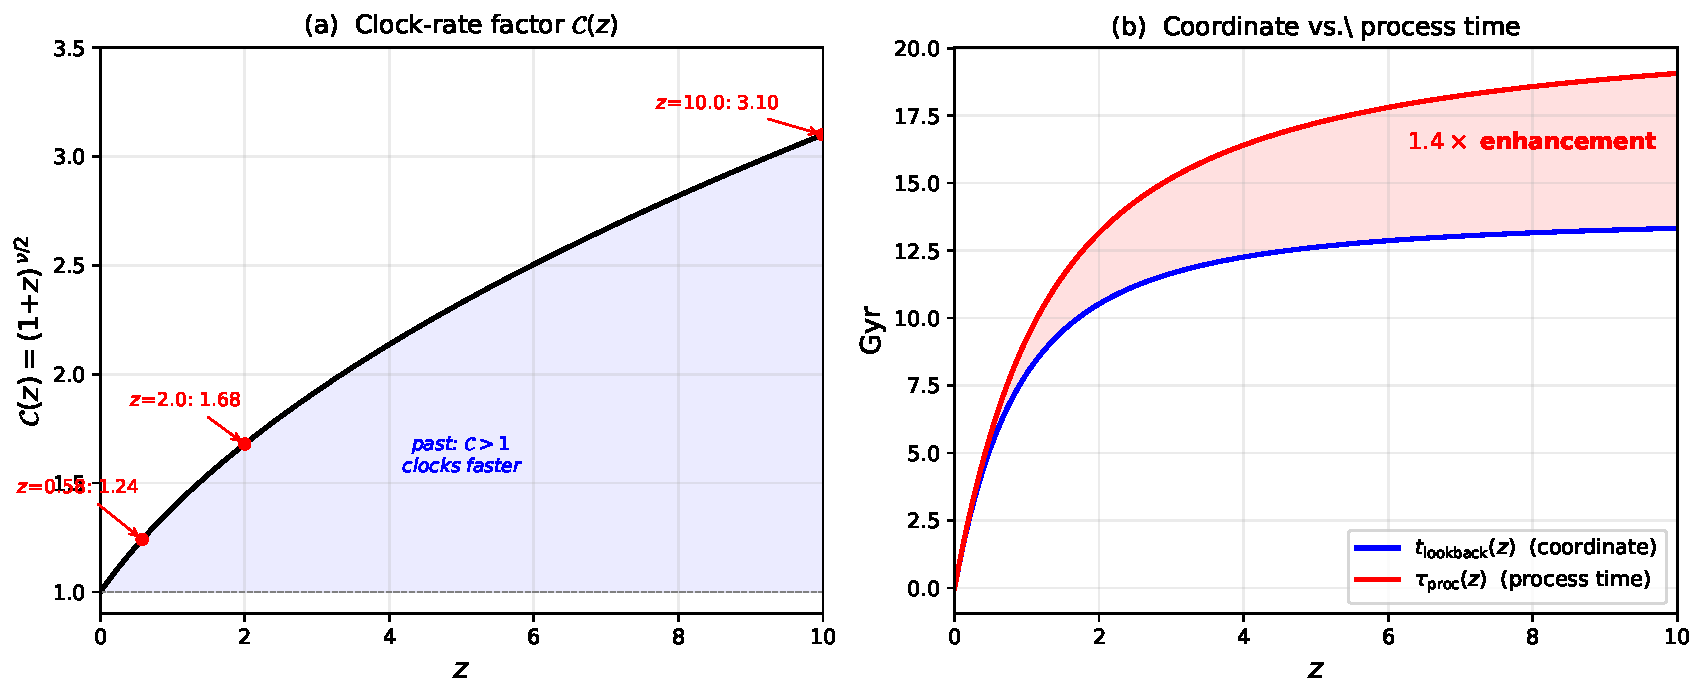
\includegraphics[width=\textwidth]{PDF/fig_Cz_processtime.pdf}
\caption{%
(a)~Background history factor
$\mathcal{C}(z)=(1{+}z)^{\nu/2}$ with $\nu=0.94$,
a power-law approximation calibrated to the companion MOND
paper benchmark $\mathcal{C}(10)\approx 3.1$; the full
$\mathcal{C}(z)$ from the coupling-ratio formula
(Eq.~\ref{eq:Cfactor_app18}) has a more complex shape at
intermediate $z$.
Red dots mark specific benchmarks.
(b)~Coordinate lookback time (blue) versus cumulative process time
(red) from $z=0$ to $z=10$.  The shaded region is the
enhancement due to the faster process-clock rate in the past.
Both panels use standard $\Lambda$CDM $H(z)$ with
$\Omega_m=0.315$, $H_0=67.4\;\mathrm{km\,s^{-1}\,Mpc^{-1}}$.
\label{fig:Cz}}
\end{figure}

\section{Rate conversion and the no-double-counting rule}
\label{sec:what_counts_app18}

The distinction between $t_{\mathrm{lb}}$ and $\tau_{\mathrm{proc}}$ is
not cosmetic.  Whenever a phenomenon is governed by cumulative
pressure-controlled matter-sector evolution, the relevant history integral must be written in
process time.

\paragraph{Intrinsic-rate formulation.}
If $X$ is a cumulative quantity whose microscopic law is fundamental per
unit process time,
\begin{equation}
  \frac{dX}{d\tau_{\mathrm{proc}}} = \mathcal{R}_{\mathrm{int}},
  \label{eq:intrinsic_rate_app18}
\end{equation}
then the observer-frame rate is
\begin{equation}
  \frac{dX}{dt}
  = \frac{d\tau_{\mathrm{proc}}}{dt}\,\mathcal{R}_{\mathrm{int}}
  = \mathcal{C}(z)\,\mathcal{R}_{\mathrm{int}}.
  \label{eq:rate_convert_app18}
\end{equation}
Likewise the total accumulated history is
\begin{equation}
  X(t_2)-X(t_1)
  = \int_{t_1}^{t_2}\mathcal{R}_{\mathrm{int}}\,d\tau_{\mathrm{proc}},
  \label{eq:history_rule_app18}
\end{equation}
not $\int \mathcal{R}_{\mathrm{int}}\,dt$.

\paragraph{No-double-counting rule.}
Equation~\eqref{eq:rate_convert_app18} must be used only when the
underlying law is intrinsic to process time.  If a source law has already
been derived directly in the observer's time variable $t$, then an extra
factor $d\tau_{\mathrm{proc}}/dt$ must \emph{not} be inserted again.
Otherwise one counts the same clock conversion twice.  Appendix~18
therefore supplies the conversion operator and the criterion for its
legitimate use; it does not authorize blind multiplication of every
observer-frame rate by $\mathcal{C}(z)$.

\paragraph{Rate-variable tagging.}
Before applying Eq.~\eqref{eq:rate_convert_app18}, one must first identify
the time variable in which the relevant rate or power has been defined.
Dependence on $m_{\mathrm{eff}}$, $\mathcal{P}_{\mathrm{tail}}$, or another
$\phi$-dependent quantity is not by itself sufficient: the quantity may
already have been written per coordinate time or inferred from an
observer-frame rate.  The bookkeeping rule is:
\begin{center}
\small
\begin{tabular}{@{}p{0.22\textwidth}p{0.27\textwidth}p{0.22\textwidth}p{0.20\textwidth}@{}}
\hline
\textbf{Rate tag} & \textbf{Meaning} & \textbf{Conversion} & \textbf{Check} \\
\hline
Intrinsic/process-time rate &
Fundamental microscopic law per $d\tau_{\mathrm{proc}}$. &
Use $dX/dt=\mathcal{C}(z)\,dX/d\tau_{\mathrm{proc}}$. &
Apply one factor only. \\
Local proper-time rate &
Microscopic or local laboratory rate per local clock. &
Use the local metric clock law, then coarse-grain cosmologically only if needed. &
Do not mix local and FLRW conversions. \\
Coordinate/cosmic-time rate &
Source law already written with $\dot X=dX/dt$. &
No extra $\mathcal{C}(z)$ factor. &
The dot fixes the time variable. \\
Observer-calibrated/rest-frame rate &
Rate inferred from observed spectra, light curves, or population modelling. &
No post-multiplication by $\mathcal{C}(z)$ unless rederived from an intrinsic law. &
Keep standard metric time dilation. \\
\hline
\end{tabular}
\end{center}

Thus background FLRW distances, the linear CMB sector, and the
Einstein--Boltzmann evolution remain tied to the standard cosmic-time
description of Appendix~9.  Pressure-controlled matter-sector histories
use process time only after their rates have been tagged as intrinsic
process-time laws.

\paragraph{Application map.}
The same tagging rule separates the main uses of process time in the
framework:
\begin{center}
\small
\begin{tabular}{@{}p{0.17\textwidth}p{0.18\textwidth}p{0.19\textwidth}p{0.20\textwidth}p{0.17\textwidth}@{}}
\hline
\textbf{Application} & \textbf{Rate variable} & \textbf{Conversion} & \textbf{Double-counting check} & \textbf{Status} \\
\hline
Vortex maturation / MOND $a_0$ lag &
$H_{\mathrm{eff}}$ is the coordinate-time memory average; $H_{\mathrm{eff,proc}}$ is a refinement. &
Use the coordinate-time average in the main local-galaxy calibration; use process weighting only for a declared process-rate law. &
Do not replace $H_{\mathrm{eff}}/H_0$ by $\mathcal{A}$. &
Quantitative companion result. \\
Process-age factor $\mathcal{A}(z)$ &
Cumulative diagnostic $\tau_{\mathrm{proc}}/t_{\mathrm{lb}}$. &
Compute from $\int \mathcal{C}(t)\,dt$. &
It is not a Hubble-rate ratio. &
Bookkeeping diagnostic. \\
JWST high-$z$ galaxies &
Stellar-evolution, star-formation, and assembly rates. &
Convert only rates shown to be intrinsic process-time rates. &
Do not simply divide inferred ages by $\mathcal{A}(z)$. &
Potential mitigation only. \\
Tail accumulation / dark-energy source &
Tail power $\mathcal{P}_{\mathrm{tail}}$ with a declared time variable. &
R.2 fixes the perturbative pressure scaling $\mathcal{C}^4$; the integration measure is chosen separately. &
No automatic extra $\mathcal{C}$ factor. &
Source-law convention required. \\
Cluster halo formation and mergers &
$N\Gamma_{\mathrm{single}}$ is a local-proper-time microscopic rate; merger redistribution is local at the merger epoch. &
Use process-time conversion only in cosmological formation integrals. &
Do not apply it to the already local crossing time. &
Companion-cluster benchmark. \\
Observed transients and rest-frame rates &
Data-inferred observer/rest-frame rates. &
Use the standard metric $(1+z)$ time stretch. &
Do not post-multiply by $\mathcal{C}(z)$. &
Observational guardrail. \\
\hline
\end{tabular}
\end{center}

\section{Asymptotic future and non-termination in finite time}
\label{sec:asymptotic_app18}

The process-time framework naturally supports an asymptotic weakening of
activity.  Suppose the pressure-history factor $\mathcal{C}(t)$ remains
nonnegative and decreases monotonically as the universe relaxes.  Let a
pressure-controlled matter-sector rate have the form
\begin{equation}
  \mathcal{R}(t) = \mathcal{R}_0\,F[\mathcal{C}(t)],
  \qquad F(0)=0,
  \label{eq:Rfuture_app18}
\end{equation}
with $F$ continuous and nonnegative.  Since
$\mathcal{C}(t)=[P_{\mathrm{stat}}(t)/P_{\mathrm{stat}}(0)]^{1/2}$,
$\mathcal{C}\to 0$ would require complete depletion
$P_{\mathrm{stat}}\to 0$.  Three logical possibilities exist:
\begin{itemize}
\item if $\mathcal{C}(t)\to \mathcal{C}_\infty>0$ (pressure relaxes to a
  nonzero floor), the process approaches a nonzero asymptotic residual
  activity;
\item if $\mathcal{C}(t)\to 0$ only as $t\to\infty$ (complete depletion
  approached but never reached), then
  $\mathcal{R}(t)\to 0$ only asymptotically;
\item a finite-time exact shutdown would require
  $\mathcal{C}(t_\ast)=0$ at some finite $t_\ast$, which is not established
  anywhere in the present framework and would require complete exhaustion
  of the medium pressure in finite time.
\end{itemize}

Therefore the process-time formalism does \emph{not} support the statement
that the universe must reach an exact terminal zero state in finite
measured time.  What it supports, under monotonic pressure relaxation, is a
progressive weakening of clocks, effective masses, and tail-driven activity
that continues indefinitely.  The quiescent state---defined by the absence
of localized resonant excitations (Eq.~\ref{eq:quiescent_def})---is an
asymptotic attractor in this picture, not a state that is reached in
finite coordinate time.

\paragraph{Energy-flux arrow from the feedback mechanism.}
The tail-emission channel carries positive outgoing energy flux,
with total power
$\dot E_{\mathrm{tail}}\propto N_b\,\mathcal{P}_{\mathrm{tail}}>0$
(companion quantum paper, Sec.~5).  If this flux is coarse-grained
as entropy production in a scalar bath, its rate inherits the same
sign.  Since
$\mathcal{P}_{\mathrm{tail}}^{(\mathrm{pert})}\propto\mathcal{C}(t)^4$
(subject to the non-perturbative factor caveat in
Sec.~\ref{sec:clocklaw_app18}) and
$N_b\propto a^{-3}$, the outgoing power decreases monotonically but
never vanishes.  Process time therefore accumulates in the same
direction as this radiative/coarse-grained entropy arrow.

\paragraph{Scope of the ``derived arrow'' claim.}
The positivity $\dot\varepsilon>0$---which is what drives
the coarse-grained entropy-arrow statement and the phantom
equation of state $w<-1$---is itself a
statement that the tail-emission channel is irreversible: radiated
echo quanta propagate outward and do not refocus.  This one-way
propagation is an instance of the thermodynamic arrow, not a
derivation of it.  The content of this appendix is therefore the
weaker and more accurate claim: \emph{given} the irreversibility of
tail emission (imported from the standard second law, as in any
radiation-damping argument), the feedback mechanism aligns the
process-time arrow with the radiative/coarse-grained entropy arrow
and ties both to the medium-pressure depletion.  No separate
``arrow of time''
postulate \emph{beyond} that radiative/coarse-graining input is
required, but the appendix does not claim to derive the thermodynamic
arrow itself from first principles; a first-principles derivation
would require a statistical-mechanical analysis of the tail phase
space and is the topic of a separate work.

\section{Coordinate--process time duality}
\label{sec:duality_app18}

The combination of the clock-rate postulate, the operationally timeless
quiescent state (Sec.~\ref{sec:op_time_app18}), and the asymptotic
weakening of Sec.~\ref{sec:asymptotic_app18} produces a structural
duality between two natural time measures.

\paragraph{Definitions.}
Let $T_{\mathrm{ext}}$ denote coordinate (FLRW cosmic) time and
$T_{\mathrm{int}}$ denote cumulative process time
$\tau_{\mathrm{proc}}=\int\mathcal{C}(t)\,dt$.  For the past and
future half-lines:
\begin{align}
  T_{\mathrm{ext,\,past}} &= t_0 \simeq 14.7\;\mathrm{Gyr}
    &&(\text{finite}),
  \label{eq:Text_past}\\[4pt]
  T_{\mathrm{int,\,past}} &:\;
    \text{operationally undefined (quiescent medium, no resonant clock)}
    &&(\text{unbounded}),
  \label{eq:Tint_past}\\[4pt]
  T_{\mathrm{ext,\,future}} &= \int_{t_0}^{\infty}dt = \infty
    &&(\text{de~Sitter}),
  \label{eq:Text_future}\\[4pt]
  T_{\mathrm{int,\,future}} &= \int_{t_0}^{\infty}\mathcal{C}(t)\,dt
    &&(\text{finite if }\mathcal{C}\to 0\text{ fast enough}).
  \label{eq:Tint_future}
\end{align}

\paragraph{The duality.}
To avoid conflating the mathematical value of the process-time
integral with its operational status, we present the four entries with
the process-time column split into its ``mathematical'' and
``operational'' readings:
\begin{center}
\renewcommand{\arraystretch}{1.4}
\begin{tabular}{@{}lccc@{}}
\toprule
  & External (coordinate) & Process time (math.\ integral) & Process time (operational) \\
\midrule
Past   & finite ($t_0\simeq 14.7$ Gyr)
       & finite ($\approx 20$ Gyr)$^{\flat}$
       & undefined$^{*}$ \\
Future & unbounded ($\infty$)
       & finite$^{\dagger}$ ($T_{\mathrm{int,\,future}}$)
       & well-defined while $\mathcal{R}_{\mathrm{tail}}>0$ \\
\bottomrule
\end{tabular}
\end{center}
\noindent
{\footnotesize $^{*}$``Undefined'' means that no resonant clock exists
before excitations form (Sec.~\ref{sec:op_time_app18}): there is no
physical process whose microscopic rate can register the passage of
pre-resonance epoch.\par
$^{\flat}$The pre-resonance mathematical integral
$\int_0^{z_{\max}}\mathcal{C}\,dz/[(1{+}z)H]$ is finite under the
fiducial closure used below; the value $\approx 20\;\mathrm{Gyr}$ is
given in the present-day normalization, $t_\star=t_0$
(Sec.~\ref{sec:flrw_vs_process_app18}).\par
$^{\dagger}$Conditional: finiteness requires $\mathcal{C}(t)\to 0$
fast enough for the integral to converge; see the convergence
condition below.}

\medskip\noindent
The diagonal structure is then between \emph{operational} entries:
the operational past is undefined while the operational future is
well-defined, and vice versa for the mathematical integrals (both
finite, one unconditionally, the other conditionally).  This is a
conjectured duality: it holds provided (i)~the convergence condition
on $T_{\mathrm{int,\,future}}$ is satisfied (open in the current
closure, see below) and (ii)~the pre-resonance regime is truly
clock-less at the microscopic level (accepted here as a working
ontology).  In particular, the coordinate age of the universe $t_0$
and the remaining operational process-time budget occupy dual
positions under this interpretation.

\paragraph{The present epoch as the crossover.}
By construction, $\mathcal{C}(t_0)=1$: the process clock and the
coordinate clock tick at the same rate \emph{today}.  In the past
$\mathcal{C}>1$ (faster process clock); in the future $\mathcal{C}<1$
(slower process clock).  The present epoch is the unique crossover point
where the two time measures coincide.  The identity
$\mathcal{C}(t_0)=1$ is, by itself, merely a normalization
convention ($\phi_{\mathrm{bg}}(0)\equiv 0$).  The
non-trivial physical content is that the \emph{same epoch}
at which $\mathcal{C}=1$ is also the epoch at which the
feedback equilibrium $\dot\varepsilon=3H\varepsilon$ is
satisfied and $\Omega_m\sim\Omega_\Lambda$; this triple
coincidence is a consequence of the self-consistent dynamics,
not of the normalization choice.

\paragraph{Relation to the coincidence problem.}
The standard cosmological coincidence problem asks why
$\Omega_{\mathrm{m}}\sim\Omega_{\Lambda}$ precisely now.  In the
ISPG feedback framework the echo-background energy density
$\rho_{\mathrm{vac}}$ is estimated, on the perturbative tail-power
branch, by the self-consistent equilibrium
$\dot\varepsilon = 3H\varepsilon$ (companion quantum paper,
Eq.~(6.14)).  The same equilibrium condition is tied to
$\mathcal{C}=1$ at the epoch where the balance is achieved:
matter--vacuum equality, the crossover of process time and coordinate
time, and the $\rho_{\mathrm{vac}}\sim 10^{-121}$
echo-background scale can be read as coupled consistency checks, not
as a completed first-principles solution of the full
cosmological-constant problem.

\paragraph{Scope of this reduction.}
Calling these three statements ``three readings of one condition''
should be read in the sense of \emph{consistency-check coupling}, not
of \emph{prediction from first principles}.  Specifically:
\begin{itemize}
\item The identity $\mathcal{C}(t_0)=1$ is, as noted above,
  a normalization convention ($\phi_{\mathrm{bg}}(0)\equiv 0$) rather
  than a derived value.
\item The equilibrium condition $\dot\varepsilon=3H\varepsilon$ is,
  by its definition, the locus of feedback saturation: its
  coincidence with $\mathcal{C}=1$ therefore reflects the way the
  balance and the normalization are \emph{set by the same feedback
  ODE}, not an independent prediction.
\item The numerical value $\rho_{\mathrm{vac}}\sim 10^{-121}\;M_{\rm
  Pl}^{4}$ is an \emph{output} of the feedback ODE at the fiducial
  closure parameters $(\alpha,K)$ fixed in the companion MOND paper;
  a tuning-free derivation of this scale is not performed here and
  remains an open quantitative target.
\item The present-epoch character of $\Omega_m\sim\Omega_\Lambda$
  therefore requires that the feedback attractor passes through
  $\mathcal{C}=1$ at the observed value of $H_0$; showing that this
  selection is natural (i.e.\ independent of the initial conditions
  of the ODE) is likewise open.
\end{itemize}
Understood in this sense, the ``single self-consistency condition''
is a structural statement about the feedback picture, not a
derivation of the observed dark-energy scale from first principles;
a proof that the scale $10^{-121}$ is selected without tuning is the
topic of a separate work.

\paragraph{Convergence condition.}
The finiteness of $T_{\mathrm{int,\,future}}$ requires
$\mathcal{C}(t)\to 0$ sufficiently fast.  If $\mathcal{C}(t)\sim
t^{-\alpha}$ at late times, the integral converges for $\alpha>1$.
The dark-energy equation of state $w<-1$ (source-driven phantom)
reflects $\dot\varepsilon>0$ at all epochs (the echo background never
stops growing), so $\phi_{\mathrm{bg}}$ continues to decrease and
$\mathcal{C}$ continues to fall even in the de~Sitter phase.  The
sign of this branch follows from the positive source term, while
the size of $\delta w_0$ remains conditional on the tail-power
normalization; current DESI CPL fits therefore provide a mixed
test of the branch rather than a confirmation.  Whether
the late-time falloff is fast enough for convergence depends on the
asymptotic solution of the feedback ODE beyond the de~Sitter
saturation regime; this calculation remains open and is identified
as a quantitative target for future work.

\paragraph{Active-phase budget.}
Even if $\mathcal{C}$ freezes at a nonzero floor $\mathcal{C}_\infty$
(making the total integral diverge), the \emph{active} portion of
the future process-time budget---the part during which $\mathcal{C}$
is still changing appreciably---is finite and computable.
Define
\begin{equation}\label{eq:tau_active_def}
  \tau_{\mathrm{active}}
  := \int_{t_0}^{\infty}
     \bigl[\mathcal{C}(t)-\mathcal{C}_\infty\bigr]\,dt.
\end{equation}
In the de~Sitter phase the baryon sources that drive the feedback
are diluted as $n(t)\propto e^{-3H t}$; because the source power density
$\dot\varepsilon\propto n\,\mathcal{P}_{\mathrm{tail}}$ shuts off
on the timescale $1/(3H)$, the deviation
$\mathcal{C}(t)-\mathcal{C}_\infty$ likewise decays as
$e^{-3H(t-t_0)}$ at late times.  During this transient
$\mathcal{C}(t_0)=1$, so process time $\approx$ coordinate time and
\begin{equation}\label{eq:tau_active}
  \tau_{\mathrm{active}}
  \;\sim\; \int_{0}^{\infty}
           (1-\mathcal{C}_\infty)\,e^{-3Ht'}\,dt'
  \;=\; \frac{1-\mathcal{C}_\infty}{3H_0}
  \;\sim\; \frac{1}{3H_0}
  \;\approx\; 4\text{--}5\;\mathrm{Gyr}.
\end{equation}
The full transition from $\mathcal{C}=1$ to the asymptotic floor
occupies a few $e$-folding times, so the total active-phase
duration is of order $H_0^{-1}\simeq t_0\simeq 14.5\;\mathrm{Gyr}$.
After that, $\mathcal{C}$ is effectively frozen and no further
pressure depletion occurs: coordinate time continues but process
time accumulates at a constant, residual rate.

The coordinate age $t_0$ and the active-phase process-time budget
are therefore set by the same physical scale $H^{-1}$, confirming
the anti-diagonal structure of the duality table on purely
dynamical grounds.

\paragraph{Physical reading.}
If the duality is exact, the universe has no absolute beginning and
no absolute end: it has a finite coordinate past that is an
unbounded process past (no operational clock before resonances), and
an unbounded coordinate future that is a finite process-time future
(asymptotically vanishing activity).  The ``Big Bang'' and the
``heat death'' are not terminal events but transitions between the
two temporal regimes, and the present epoch is the symmetric midpoint
where both descriptions agree.

\paragraph{Two-observer comparison.}
Every physical observable in the bi-conformal framework can be
expressed in two equivalent languages---the coordinate frame
(coordinate observer, time variable $t$) and the local process frame
(local observer, time variable $\tau$).  The two are related by
the clock-rate postulate and its reciprocal rod postulate:
\begin{center}
\renewcommand{\arraystretch}{1.4}
\begin{tabular}{@{}lcc@{}}
\toprule
Quantity & Coordinate description & Local process description \\
\midrule
Time element & $dt$ & $d\tau = e^{\phi/2}\,dt$ \\
Length element & $d\sigma$ & $d\ell = e^{-\phi/2}\,d\sigma$ \\
Speed of light & $c_{\mathrm{coord}} = c\,e^{\phi}$ & $c_{\mathrm{local}} = c$ \\
Frequency & $\omega$ & $\omega_{\mathrm{local}} = \omega\,e^{-\phi/2}$ \\
Effective mass & $m_0\,e^{\phi/2}$ & $m_0$ (locally undetectable) \\
Tail power & $\mathcal{P}\propto e^{2\phi}$ & $\mathcal{P}_{\mathrm{local}}\propto 1$ \\
\bottomrule
\end{tabular}
\end{center}
\noindent
The local observer measures $c=\mathrm{const}$,
$m_0=\mathrm{const}$, $\mathcal{P}=\mathrm{const}$: all local
physics is $\phi$-independent.  The proof requires only the table
entries above.  The local speed of light is
\begin{equation}\label{eq:clocal_proof_app18}
  c_{\mathrm{local}}
  = \frac{d\ell}{d\tau}
  = \frac{e^{-\phi/2}\,d\sigma}{e^{\phi/2}\,dt}
  = \frac{d\sigma}{dt}\,e^{-\phi}
  = c_{\mathrm{coord}}\,e^{-\phi}
  = c\,e^{\phi}\,e^{-\phi}
  = c.
\end{equation}
The mass ratio of any two particle species $A,B$ is
\begin{equation}\label{eq:massratio_proof_app18}
  \frac{m_{\mathrm{eff}}^A}{m_{\mathrm{eff}}^B}
  = \frac{m_0^A\,e^{\phi/2}}{m_0^B\,e^{\phi/2}}
  = \frac{m_0^A}{m_0^B},
\end{equation}
and the frequency ratio of any two oscillators likewise:
$\omega_{\mathrm{local}}/\omega_{\mathrm{local}}'
= \omega/\omega'$.
In summary, every dimensionless observable is $\phi$-invariant:
\begin{equation}\label{eq:local_undet_app18}
  \frac{c_{\mathrm{local}}}{c} = 1,\qquad
  \frac{m_{\mathrm{eff}}^A}{m_{\mathrm{eff}}^B}
    = \frac{m_0^A}{m_0^B},\qquad
  \frac{\omega_{\mathrm{local}}}{\omega_{\mathrm{local}}'}
    = \frac{\omega}{\omega'}.
\end{equation}
No local experiment can detect a uniform shift of $\phi$;
only comparisons across different epochs---where
$\phi_{\mathrm{bg}}$ has changed---reveal the pressure history.
This is the local undetectability theorem
(companion quantum paper, Sec.~4.3).
The external observer sees all three quantities change with $\phi$.
Neither frame is privileged; they are connected by the conformal
rescaling $e^{\phi/2}$.

\noindent Applied to cosmological history ($\phi\to\phi_{\mathrm{bg}}(z)$):
\begin{itemize}
\item \textbf{Coordinate view of the future}: process clocks slow down
  ($d\tau/dt \to 0$), effective masses shrink, tail emission weakens.
  A finite amount of resonant-sector activity is stretched over infinite
  coordinate time.
\item \textbf{Local-process view of the future}: all local measurements
  remain ``normal'' ($c=c$, $m_0=m_0$), but the universe empties
  (de~Sitter dilution).  The observer has infinite coordinate time
  ahead but with progressively less content per process-time unit.
\item \textbf{Coordinate view of the past}: process clocks were fast,
  masses were larger, emission was stronger.  An unbounded amount of
  resonant-sector activity is compressed into the finite coordinate interval
  $t_0$.
\item \textbf{Local-process view of the past}: all local measurements were
  ``normal,'' but the universe was denser, hotter, and richer in
  events per process-time unit.  Looking back, the local observer
  sees an ever-denser past with no operational beginning.
\end{itemize}
The two descriptions are physically equivalent: ``time runs out''
(coordinate description) and ``content runs out'' (local process description) are dual
translations of the single equation $d\tau = e^{\phi/2}\,dt$.

\section{Existing quantitative uses already present in the framework}
\label{sec:existing_uses_app18}

Although the present appendix is the first place where the principle is
collected systematically, the framework already uses it in concrete
applications:
\begin{enumerate}
\item \textbf{Enhanced vortex formation time.}
  The companion MOND paper (Sec.~5.5) uses the coordinate-time
  vortex-lag diagnostic $H_{\mathrm{eff}}$ in the local-galaxy
  calibration.  For $z_{\mathrm{form}}=0.58$,
  $H_{\mathrm{eff}}/H_0\approx 1.15$ (companion MOND paper,
  Eq.~(5.15) and Table~1).  With the same pressure-history profile,
  the process-time weighted diagnostic is
  $H_{\mathrm{eff,proc}}/H_0\approx 1.16$, while the cumulative
  process-age factor is $\mathcal{A}(0.58)\approx 1.11$.
  These are related diagnostics but not interchangeable.
\item \textbf{JWST high-redshift galaxies.}
  The same logic can reduce the required intrinsic development time
  for rates that are genuinely process-time controlled.  It does not,
  by itself, authorize dividing stellar-population or assembly ages by
  $\mathcal{A}(z)$.  A quantitative JWST age claim requires an explicit
  map from stellar-evolution, star-formation, and assembly rates to the
  appropriate time variable.
\item \textbf{Cluster-merger timing.}
  The process-time integral is used only for the formation history
  of a medium-memory halo whose microscopic build-up rate has been
  tagged as local-proper-time/process-controlled.  Merger crossing
  and redistribution times at the observed epoch remain local
  merger-time quantities (companion MOND paper, Sec.~8).
\item \textbf{Coupling-enhancement ratio.}
  The companion MOND paper (Eq.~(5.23)) derives the ratio
  $e^{2\phi(z)}/e^{2\phi(0)}$ from the quantum feedback ODE.
  This is precisely the perturbative $\mathcal{C}(z)^4$ factor of
  Sec.~\ref{sec:clocklaw_app18}.  This factor is the pressure-amplitude
  scaling of the perturbative tail channel; it does not by itself
  specify whether a tail power is defined per process time, local
  proper time, or coordinate time.  The integration measure must be
  chosen only after that convention is fixed, so no additional
  $\mathcal{C}(z)$ factor is inserted automatically.  The
  identification relies on reading the feedback-ODE $\phi$---a
  microscopic oscillon-averaged quantity---as the coarse-grained
  cosmological $\phi_{\mathrm{bg}}$ at a coarse-graining scale
  $\ell_{\mathrm{cg}}$ that is large compared to individual oscillon
  sizes but small compared to cosmological gradients.  Within this
  appendix we adopt this identification as a postulate of the
  coarse-graining scheme; a quantitative check that the $\ell_{\mathrm{cg}}$
  chosen in the MOND paper is compatible with the cosmological
  volume-averaging used in Eq.~\eqref{eq:phibg_def_app18} is the
  topic of a separate work.
\end{enumerate}

\paragraph{Status of the listed uses.}
The four applications above are quantitative \emph{uses} of the
process-time principle within the larger ISPG programme; they are
not independently verified in Appendix~18.  Their numerical
robustness depends on the MOND-companion closure (items 1, 2, 4) and
on the cluster-merger modelling (item 3), both of which are the
topic of the companion papers.  This appendix supplies only the
clock-rate rule and the conversion operator; quantitative
conclusions drawn from the table above should be read as
``existing uses at the stated reference,'' not as
Appendix-18-internal results.

\section{Relation to other approaches to the nature of time}
\label{sec:comparison_app18}

The view that time is not a background but an operational or
emergent quantity has precedents in several traditions.
Barbour's timeless mechanics~\cite{Barbour1999} eliminates time
altogether, treating it as an illusion arising from correlations
between static configurations.
Rovelli's thermal time hypothesis~\cite{ConnesRovelli1994}
derives a time flow from the thermodynamic state of a quantum
system via the Tomita--Takesaki theorem.
Whitehead's process philosophy identifies reality with
``actual occasions'' rather than enduring substances, making
becoming prior to being~\cite{Whitehead1929}.
Penrose's conformal cyclic cosmology~\cite{Penrose2010} exploits
the conformal equivalence between the remote future (where all
mass has vanished) and a new Big Bang.

The ISPG process-time framework shares conceptual ground with
each of these: time is operational (Barbour), tied to
thermodynamic state (Rovelli), defined by process (Whitehead),
and exhibits a future--past structural symmetry (Penrose).
The distinguishing feature is not that ISPG is the first to
propose a quantitative time equation---Rovelli's thermal time,
for instance, gives a precise modular flow---but that ISPG
ties its clock law $d\tau = e^{\phi/2}\,dt$ to a single
identified physical mechanism (pressure-dependent clock rate
from the bi-conformal metric), from which the present appendix
assembles a structured programme rather than a completed set of
derivations: the duality table
(Sec.~\ref{sec:duality_app18}, conditional on the convergence of
$T_{\mathrm{int,\,future}}$), the entropy-arrow alignment
(understood as an alignment with the imported second law rather
than a derivation of it), and the feedback-equilibrium reading of
the coincidence problem (a structural reduction of three
coincidences to a single self-consistency condition whose
numerical output $\rho_{\mathrm{vac}}\sim 10^{-121}$ depends on the
closure parameters of the companion MOND paper).  Each of these
items is in a distinct stage of maturity, and a sharper
identification of observational signatures that would distinguish
the ISPG process-time picture from Rovelli-type thermal time or
Penrose-type cyclic cosmology is itself an open target of the
programme rather than a completed result of this appendix.

\section{Takeaway}
\label{sec:takeaway_app18}

The ISPG framework contains a precise pressure-history time weighting that
follows directly from the clock-rate postulate:
\begin{equation}
  d\tau_{\mathrm{proc}} = \mathcal{C}(z)\,dt.
\end{equation}
This does not modify the homogeneous FLRW metric clock of Appendix~9:
$\phi_0=0$ constrains the metric, while $\phi_{\mathrm{bg}}(z)$ tracks
the coarse-grained thermodynamic state of the medium.  Whenever the past
pressure was higher than the present one, the cumulative process duration
exceeds the naive lookback time measured by today's clocks.  This weighting
must be inserted through the explicit rate-conversion rule, without double
counting.

The framework further reveals a coordinate--process time duality
(Sec.~\ref{sec:duality_app18}): the finite coordinate age $t_0$ and
the finite remaining process-time budget
$T_{\mathrm{int,\,future}}$ occupy anti-diagonal positions in the
past/future table, with the present epoch as the unique crossover
where $\mathcal{C}=1$.  If the convergence of $T_{\mathrm{int,\,future}}$
is confirmed, the dark-energy scale estimate, the coincidence problem,
and the arrow of time become linked consistency checks of one feedback
condition rather than three independent puzzles.  This is a conditional
interpretive unification, not a completed solution of the full
cosmological-constant problem.

\end{document}
